\documentclass{article}



\usepackage{arxiv}

\usepackage[utf8]{inputenc} % allow utf-8 input
\usepackage[T1]{fontenc}    % use 8-bit T1 fonts
\usepackage{hyperref}       % hyperlinks
\usepackage{url}            % simple URL typesetting
\usepackage{booktabs}       % professional-quality tables
\usepackage{amsfonts}       % blackboard math symbols
\usepackage{nicefrac}       % compact symbols for 1/2, etc.
\usepackage{microtype}      % microtypography
\usepackage{lipsum}		% Can be removed after putting your text content
\usepackage{graphicx}
\usepackage{natbib}
\usepackage{doi}
\usepackage{amsmath,amsfonts,amssymb,amsthm}
\usepackage{enumitem}
\usepackage{adjustbox}
\usepackage{array,ragged2e}
\usepackage{longtable}
\usepackage{pdflscape}
\usepackage{makecell}
\usepackage[font=small]{caption}
\usepackage[justification=centering]{caption}
\usepackage{booktabs}
\usepackage{chngcntr} % for local labelling
\usepackage{mathtools, nccmath}
\usepackage{physics}
\usepackage{subfig}
\usepackage{fancyvrb}
\usepackage{tcolorbox} % Grey Box Hightlight
\usepackage{color}
\usepackage{float}
\usepackage[fontsize=12pt]{fontsize}
\setlength\parindent{0pt}


\graphicspath{{../images/}} % NOTE: Put all your figures in this directory.

\title{Understanding Double Descent In the Case of Simple Linear Regression}

\author{
	Zion Sheng (NetID: zs144)\\
	Department of Electrical and Computer Engineering\\
	Duke University\\
	Durham, NC 27708 \\
	\texttt{zion.sheng@duke.edu} \\
}

\date{} % remove the date

% Uncomment to override  the `A preprint' in the header
% \renewcommand{\headeright}{Technical Report}
\renewcommand{\undertitle}{CS590 (Theory in ML) Final Project Report}
% \renewcommand{\shorttitle}{\textit{arXiv} Template}

%%% Add PDF metadata to help others organize their library
%%% Once the PDF is generated, you can check the metadata with
%%% $ pdfinfo template.pdf
\hypersetup{
	pdftitle={A template for the arxiv style},
	pdfsubject={machine learning},
	pdfauthor={Zion Sheng},
	pdfkeywords={machine learning, double descent, bias-variance trade-off, P300 speller},
}

\begin{document}
\maketitle

\begin{abstract}
	The bias and variance tradeoff used to dominate the model design in the classic machine learning era. The traditional theory believes overly complicated models with low training risk tend to have weak generalizability (a high test risk). However, recent studies have justified the value of overparameterized models since they can achieve both zero training risk and low test risk. The new pattern behind this phenomenon is called "Double Descent", where practitioners and theoreticians find that there is a second descent after the model enters the over-parameterized regime, while the underfitting and overfitting are in the under-parameterized regime. This paper tries to understand and investigate this phenomenon in a simple linear regression setting. Specifically, we fix the model size and vary the sample size to reproduce the double descent curve on some synthesized data based on \cite{nakkiran2019more}. After we successfully reproduce the result, we then train the same linear regression model but with regularization to compare the performances. Finally, we explore the prospects and limitations of "Double Descent" on the application of the P300 speller, which is our research interest outside of theory learning in this course.
\end{abstract}


% keywords can be removed
\keywords{machine learning, double descent, bias-variance tradeoff, P300 BCI}


\section{Introduction} \label{Introduction}
\subsection{Traditional view of bias and variance tradeoff} \label{traditional}
\vspace{-1mm}
Bias and variance tradeoff is one of the most important concepts in classic machine learning. This rule regulates model test risks with different model complexity. To formalize these concepts, suppose we are given $n$ training samples $(\mathbf{x}_i, y_i) \in \mathbb{R}^d \times \mathbb{R}$, where $\mathbf{x}_i$ is the features for one data point and $y_i$ is the corresponding response. Our learning task is to train a model $f_n: \mathbb{R}^d \to \mathbb{R}$ such that we can accurately predict response $y$ given the features $\mathbf{x}$ of any input data points. In practice, the strategy is that we want to maximize the test accuracy while maintaining the training accuracy at a high level. The test accuracy, or relatively the test risk, indicates how well the model can generalize on unseen data, which is not something we can directly control as the training accuracy. We define $l$ as the function to quantify the loss between predictions and the ground truth. Specifically, during training, we use empirical risk minimization (ERM) or some other derivative algorithm to find a proper model $f$ in some function class $\mathcal{H}$ such that it has the minimal empirical risk (also called training loss) $\frac{1}{n}\sum_{i=1}^nl(f(\mathbf{x}_i), y_i)$. Although the training set and testing set are generated on the same distribution $\mathcal{P}$, the concern is that the $f$ derived by ERM may not simultaneously minimize the true risk (also called test risk) $\mathbb{E}[l(\mathbf{x}), y|(\mathbf{x}, y) \sim \mathcal{P}]$. The conventional bias and variance tradeoff believes there are two stages when we look at the change of training risk and test risk: underfitting and overfitting \cite{hastie2009elements}. If the model is too simple (i.e., a small model class $\mathcal{H}$ capacity), all participants in $\mathcal{H}$ tend to underfit the training set, resulting in both a low training risk and a low test risk. On the other hand, if the model is overly complicated (i.e., a big model class $\mathcal{H}$ capacity), then models will overfit the training data and generate badly on new samples, so the test risk is still high this time but the training risk is optimized. Generally, the training risk decreases as the model becomes more complex, whereas the test risk reduces first and then bounces back. Why do we have a U-shaped curve for the change of test risk? This is because it can be decomposed into three parts: an increasing bias, a decreasing variance, and a constant irreducible error in \cite{neville2008bias}. Therefore, between the two stages, there exists a balanced point where the model is neither too simple nor too complicated, leading to the ideal training risk and test risk. Another widespread rule of thumb is that: don't overfit the model to a zero training risk because it will definitely harm its performance during testing.

\vspace{-2mm}
\subsection{Modern viewpoint: Double Descent} \label{modern}
\vspace{-1mm}
However, modern practice has started to extend the previous view on the choice of models. Practitioners find that modern machine learning techniques, such as deep neural networks, can still perform relatively well on testing data even if they have already achieved low or even zero training risk. For these complicated neural networks, the number of weights (parameters) is usually much more than the number of samples so that the model can easily reach zero training risk. We name such phenomena of those heavily overparameterized models as "interpolation", which was first officially proposed by \cite{belkin2019reconciling}. This sparked the beginning of a wave of research in this area, and more interesting findings were revealed. \cite{nakkiran2019more} turns the attention to the performance of the fixed model size with different sample size and derive a similar conclusion. In \cite{nakkiran2021deep}, they further explore more different training settings and experiment with the most cutting-edge deep neural networks such as the transformer, which overall provides an in-depth and surrounding summarization of the double descent. \cite{zhang2021understanding} suggested that deep neural networks are competent even for classification tasks with data generated completely randomly. Although our focus is more on the application side, there are still many theoretical works on this topic worthy to be referred to. Works that analyze the double descent in simple settings (e.g., linear regression, random Fourier features) include: \cite{Bartlett_Long_Lugosi_Tsigler_2019}, \cite{Muthukumar_Vodrahalli_Subramanian_Sahai_2019}, \cite{Mitra_2019}, \cite{Derezinski_Liang_Mahoney_2019}, \cite{Liang_Rakhlin_2020}, \cite{Mei_Montanari_2022}. For theoretical analysis on double descent in neural networks, the related works we recommended include: \cite{d2020double} and \cite{baldassi2021unveiling}.\\

\vspace{-3mm}
Now, it's time to introduce the main character in the long line of papers we breifly covered above: double descent. We mentioned it several times in the previous paragraph, and grant it the title as the updated version of the traditional bias and variance tradeoff. But what it is? And how does it reconcile with the classic theory? We will elaborate on these questions right now.\\

\vspace{-3mm}
Double descent refers to the behavior of the test risk curve when it enters the interpolating regime. Empirical evidence of many model architectures shows that, if the model becomes sufficiently over-parameterized that it starts to interpolate the training data, the U-shaped test risk curve will first surge to the peak at some point called interpolating threshold, and then immediately drop back to a comparatively low level as we keep increasing the model complexity. In other words, a second descent appears after the previous U-shaped curve. At this point, much theoretical analysis has proved that the double descent is not a coincidence, but rather it holds under many different assumptions and learning settings. The mathematical derivations to obtain the expression of loss and variance could last for several pages (such as \cite{hastie2022surprises}), so we decide to skip this here in our work as our focus is on empirical analysis, but the key reason for a second descent is that the bias and variance are different in the over-parameterize regime, and their sum (roughly the test risk) is decreasing as the model complexity increases.

\vspace{-2mm}
\subsection{Our work} \label{our}
\vspace{-1mm}
Due to the limited amount of time and computation resources, it's impossible for us to explore the double descent in the deep nerual network setting. Therefore, we choose to use simple linear regression where double descent also holds. Note that there is a big difference in the problem formalization in the context of linear regression. In deep neural networks, we can simply make the model more complex by deepening and broadening the networks to investigate the change of performance while the amount of data is fixed. However, we can't do this in linear regression because the input dimension equals to the number of model parameters. In this case, adding more parameters will also increase the sample size, leading to an increment of available information to the model. This violates the requirement of variable controls. As an alternative method, we can instead fix the model size ($d$) while changing the number of samples ($n$). The result should be same as long as the ratio $n/d$ is changed, so either tuning $d$ or $n$ shouldn't be a problem.\\

\vspace{-3mm}
The organization of this paper can be listed as follows: In Section \ref{Theoretical}, we start by setting up the linear regression problem, including the assumptions, variables naming, and model definition. Then, we will derive the closed-form solution of the weight estimation, and use the results to further derive the analytical expression of bias and variance in different regimes. In Section \ref{Experiment}, we will explain how we conducted the experiment. The visualization results and result analysis are included in Section \ref{Results}. Finally in Section \ref{Conclusion}, we investigate the possible way to apply the double descent to the development of P300 spellers, which is essentially training a classifier to classify different brain waves. This section is ended by a brief conclusion of the whole report.


\section{Theoretical Analysis} \label{Theoretical}
\subsection{Problem Setup} \label{problem}
Recall that the pattern we are trying to learn is $f: \mathbb{R}^d \to \mathbb{R}$. We define the features as $\mathbf{x}$, and the response as $y$. The training set and testing set are all both generated from the same distribution $\mathcal{P}$ where the covariates of features $\mathbf{x}$ is isotropic, i.e., $\mathbf{x} \sim \mathcal{N}(0, \mathbf{I}_d)$, where $\mathbf{I}_d$ is the identity matrix of dimension $d$. The true model is defined as:
\begin{equation}
	y = \mathbf{x}^\intercal \beta + \eta, \ \text{where} \ \eta \in \mathcal{N}(0, \sigma^2)
\end{equation}
$\beta$ is the true weights, and $\eta$ is the noise term. To simplify the analysis, we require $||\beta||_2 = 1$. Suppose we have $n$ samples $(\mathbf{x}_i, y_i)$, and we want to train a linear model $\hat{f} = \mathbf{x}^\intercal \hat{\beta}$. $\hat{\beta}$ is the learnable parameter here, and we want to find a $\hat{\beta}$ with the minimum square error on the test set. Since the features matrix is isotropic, test risk $R(\hat{\beta})$ can be expressed as:
\begin{equation}
	R(\hat{\beta}) = \mathbb{E}[(\mathbf{X} \hat{\beta} - \mathbf{y})^2|(\mathbf{X}, \mathbf{y}) \sim \mathcal{P}] = ||\beta - \hat{\beta}||^2 + \sigma^2
\end{equation} 
, where $\mathbf{X} = [\mathbf{x}_1, \mathbf{x}_2, ..., \mathbf{x}_n]^\intercal$ and $\mathbf{y} = [y_1, y_2, ..., y_n]^\intercal$. We can't directly minimize the test risk. Instead, we need to train the model and hope that it can be nicely generalized on test data. To do this, we use vanilla gradient descent as the optimization algorithm to find the model with the lowest training risk. In other words, the learning objective can be written as $\min_{\hat{\beta}} ||\mathbf{X} \hat{\beta} - \mathbf{y}||^2$. The learning task here has the closed-form solution $\hat{\beta} = \mathbf{X}^\dagger\mathbf{y}$, where $\mathbf{X}^\dagger$ is the Moore-Penrose pseudoinverse. Interestingly, $\mathbf{X}^\dagger$ has different expressions on the different $n/d$ ratio. For $n \leq d$, we call it the under-parameterized regime. Otherwise, it's over-parameterized regime. Recall that we can always derive the unique solution for the simple linear regression model when $n > d$. But when $n > d$ (interpolation), there could be multiple available solutions, so we will choose the one with the smallest $\mathcal{L}_2$ norm, i.e., $||\hat{\beta}||^2$. Therefore, the solution $\hat{\beta}$ can be expressed as:
\begin{equation}
	\hat{\beta} = \mathbf{X}^\dagger \mathbf{y} = \left\{
	\begin{aligned}
		& \arg\min_{\hat{\beta}}||\hat{\beta}||^2 \  \text{s.t.} \ \mathbf{X}\hat{\hat{\beta}} = \mathbf{y} & \text{when} \ n < d\\
		& \arg\min_{\hat{\beta}}||\mathbf{X}\hat{\beta} - \mathbf{y}||^2 & \text{when} \ n \geq d
	\end{aligned}
	\right.
\end{equation}

At this point, we can already get some intuition to foresee a peak when $n = d$. Remember the samples are noisy due to the noise term $\eta \in \mathcal{N}(0, \sigma^2)$. In the over-parameterized regime, we have multiple interpolating models, and we can find the one with the smallest $\mathcal{L}_2$ norm. However, when $n = d$, we only have one interpolating model, and the $\mathcal{L}_2$ norm of this only solution must be high to fit the noise term. As a result, the varying term in the test risk $||\beta - \hat{\beta}||^2$ must be high too. After we give a more comprehensive explanation of the bias and variance term in the next subsection, we believe readers will have a clearer understanding, even if it may seem confusing at this point. 

\subsection{Analysis on the bias and variance}\label{analysis}
According to \cite{nakkiran2021deep}, we can approximately compute the bias, variance, and test risk as follows. For the over-parameterized regime, denote $\gamma = n/d < 1$ as the over-parameterization ratio. The bias $B_n$ and variance $V_n$ can be expressed as:
\begin{align} 
	B_n &= (1 - \gamma)^2||\beta||^2\\ 
	V_n &\approx \gamma (1-\gamma)||\beta||^2 + \sigma^2\frac{\gamma}{1-\gamma}
\end{align}
The expected test risk can be approximated by the sum of the bias and variance, which is:
\begin{equation}
	\mathbb{E}[\bar{R}(\hat{\beta})] \approx (1-\gamma)||\beta||^2 + \sigma^2\frac{\gamma}{1-\gamma}
\end{equation}

For the under-parameterized regime, set $\gamma = n/d\leq< 1$ as the under-parameterization ratio. The bias $B_n$ and variance $V_n$ can be expressed as:
\begin{align} 
	B_n &= 0\\ 
	V_n &\approx \sigma^2\frac{1}{\gamma - 1}
\end{align}
In this case, the expected test risk is mainly determined by the variance term. Note that the detailed derivation is enclosed in \cite{nakkiran2021deep} and \cite{hastie2022surprises}, which are very long and beyond our mathematical ability to fully understand. We assume that the "outsourced" derivations are solidly correct (we will verify by the simulation in Section \ref{Experiment}). Having the final expressions above is sufficient for us to generate the theoretical results in the experiment below.


\section{Experiment} \label{Experiment}
\subsection{Experiment 1}
We first want to verify whether the theoretical results are correct. To do this, we fix the dimension $d$ of the linear regression model to $200$. We also pre-set the true parameter $\beta$ to an arbitrary number (the norm must be $1$) and fix the standard deviation of the noise term as $\sigma = 0.5$. Then, we select $151$ candidates of the sample size ranging from $0$ to $600$. We select more samples around the $n = 200$ since the change should be more dramatic compared to the other intervals. For each candidate, we run $40$ simulations and compute the average performance (test loss and train loss). In each simulation, we will randomly generate a train set and a test set. The randomness here makes the train risk and test risk different each time, but the trend is unveiled after averaging the $40$ simulation on each $n$.\\

\vspace{-4mm}
After affirming that the simulation aligns with the theoretical results, we try a regularized linear model with a $\mathcal{L}_2$ regularization term. As a comparison, for each $d$, we also plot its average train risk and test risk in the same graph of the vanilla linear model.

\subsection{Experiment 2}
Next, we experiment with different model sizes and noise levels by varying dimension $d$ and the standard deviation of the noise term $\sigma$. For $d$, we choose two different values: $200$ and $500$. For $\sigma$, we pick three different levels: $0.1, 0.5$, and $1.0$. Note that we select $172$ candidates ranging from $0$ to $800$ when $d = 500$. Unsurprisingly, we need to repeat the above process on the different combinations of $d$ and $n$. This time we only visualize the test risk curves. By comparing these curves, we can observe how the double descent looks like in different configurations.\\

\vspace{-4mm}
Both experiments are run on a Macbook Pro 2020 with Intel Core i5 CPU. The code was written in Python. We also tested the code on a Macbook Air 2021 with M1 CPU and ended with the same result, so the reproducibility should be guaranteed.


\section{Results} \label{Results}
Let's first look at the results of experiment 1 shown in Figure \ref{fig:1}. The right subplot is the theoretical results we derived by the expression in Section \ref{analysis}. When $n > 200$ (the under-parameterized regime), the test risk increases with less training data (the ratio $n/d$ is decreasing). The test risk diverges to $\infty$ as the ratio approaches $1^+$. Then, we will fall into the over-parameterized regime ($n \leq 200$), starting from an infinite test risk. As we keep reducing the number of samples, the test risk soon drops to a local minimum (between $n=100$ and $n=150$), and finally, it slowly grows back again and reaches $1$ when $n = 0$ (random guess). We also paint the areas representing the bias term and variance term under the test risk curve. This tells us that the non-monotonicity of test risk comes from the non-monotonicity of variance, which decreases, then increases, and then decreases again after the interpolation threshold ($n = d = 200$). Before we proceed to compare the theoretical results with the simulation, we have to emphasize that the second descent (in the context of varying the model size) appears at the left half of the curve here. Because we change the sample size while fixing the model size, the left half is the over-parameterized regime, while the right half is the under-parameterized regime. If we flip the plot horizontally, then it should look similar to those plots whose x-axis measures the model complexity (e.g. \cite{belkin2019reconciling}).\\

\vspace{-3mm}
The left subplot displays the results of the simulations. The solid blue curve depicts the change of the average test risk. If we ignore the tiny fluctuations due to the noise, we can consider it perfectly matches the theoretical test risk. The training risk curve (solid red line) is also consistent with our understanding as it keeps decreasing when the ratio $n/d$ is decreasing (from right to left on the x-axis). After it enters the over-parameterized regime, those interpolating models are guaranteed to reach zero training risk. Another interesting phenomenon is that regularization can easily fix the "risk explosion" problem when $n$ is around $d = 200$. In fact, the explosion itself is very counter-intuitive as the common belief is that "More data is better", more interestingly, this is not just for linear regression. Similar things happen on deep neural networks as well reported by \cite{nakkiran2021deep}. Nevertheless, at least we know that adding an $\mathcal{L}_2$ regularization term can eliminate this problem without significantly harming the train loss (dashed red curve) and test loss (dashed blue curve) outside the area around $200$.

\vspace{-5mm}
\begin{figure}[H]
	\centering
	\subfloat[\centering averaged simulation results]
	{{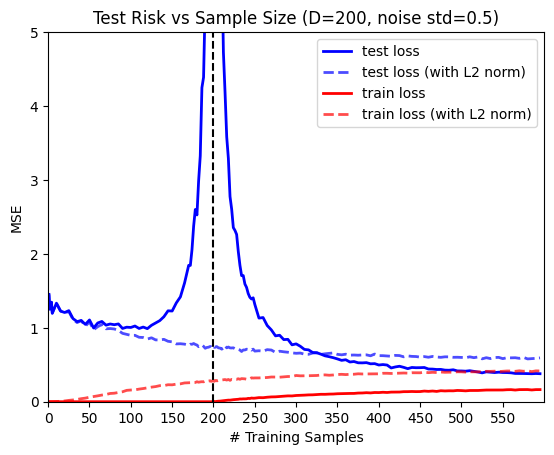
\includegraphics[width=8cm]{sim_risk_s0p5.png} }}%
	\qquad
	\hspace{-8mm}
	\subfloat[\centering theoratical results]
	{{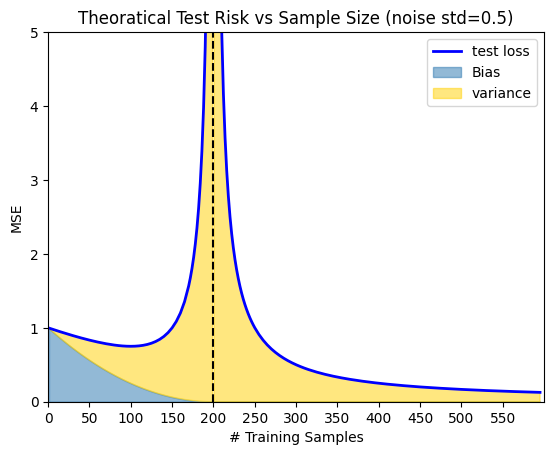
\includegraphics[width=8cm]{theo_risk_s0p5.png} }}%
	\caption{Test risk of simulation results (left) and theoratical results (right)}
	\label{fig:1}
\end{figure}

\vspace{-5mm}
Now let's turn to analyze the results of experiment 2 shown in Figure \ref{fig:2}. As we quickly scan through these curves, we can observe that the general trend of the test risk remains the same across different settings. If we alter the dimension $d$ of the model, the only change is that the interpolation threshold (the dashed black line) $n = d$ will be moved horizontally. For different noise intensities, it only affects the absolute level of the test risk. A bigger noise will cause a generally higher test risk at every sample size, but the trend (double descent) still remains. Notice that if the noise term is so strong (e.g., $\sigma = 1$), the noise term will dominate the change of the test risk when the bias term and variance term are both small. This is why the second descent (the descent in the over-parameterized regime) is not noticeable when $\sigma = 1$.

\vspace{-5mm}
\begin{figure}[H]
	\centering
	\subfloat[\centering d = 200]
	{{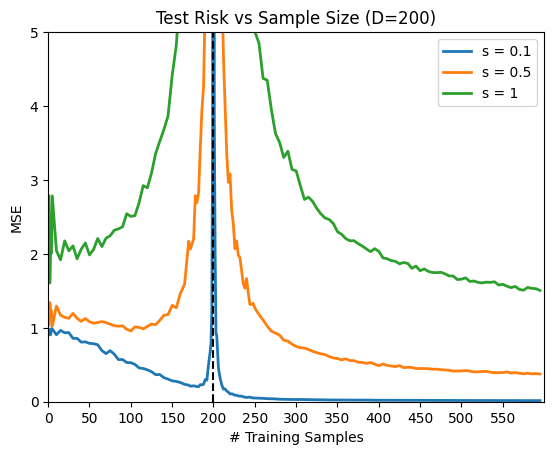
\includegraphics[width=8cm]{sim_risk_d200_diff_sigma.png} }}%
	\qquad
	\hspace{-8mm}
	\subfloat[\centering d = 500]
	{{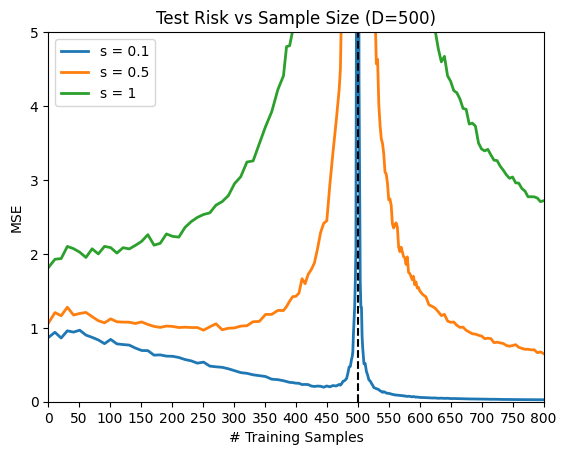
\includegraphics[width=8.1cm]{sim_risk_d500_diff_sigma.png} }}%
	\caption{Test risk of simulation results with $d=200$ (left) and $d=500$ (right)}
	\label{fig:2}
\end{figure}


\section{Discussion and Conclusion} \label{Conclusion}
\subsection{Thoughts on applying double descent on P300 spellers development}
My research concentration is on electroencephalogram (EEG) signal processing, specifically, a type of brain-computer interface (BCI) called the P300 speller. At the beginning, I was thinking to apply the findings of the double descent to the development of P300 spellers as the core task is just to train a classifier. With double descent, we can avoid choosing the bad models and bad sample sizes which leads to diverging test risks. More importantly, we hope it can direct us to find a modern solution to the development by introducing huge models and big data.\\

\vspace{-5mm}
\begin{figure}[H]
	\centering
	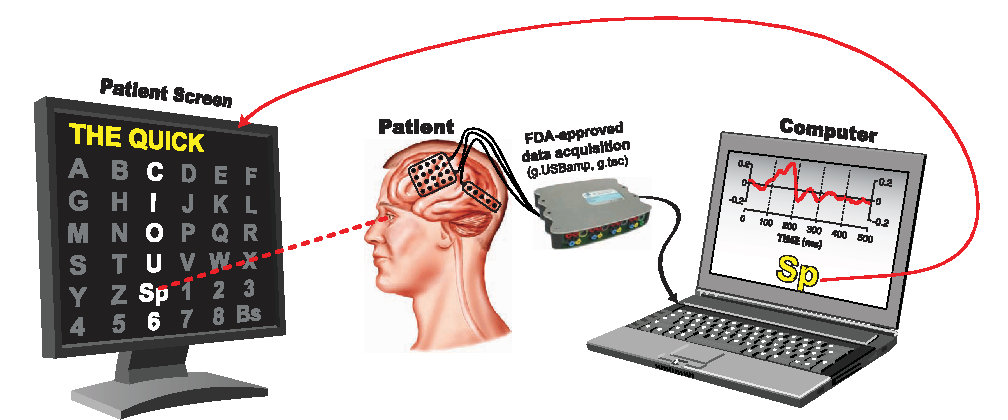
\includegraphics[width=0.6\linewidth]{p300_speller.png}
	\caption{The visualization of a P300 speller (user intereacts with the keyboard on screen while the EEG headset reads the signals and sends it to the computer to decide the desired character by the core classification algorithm)}
	\label{fig:3}
\end{figure}

\vspace{-3mm}
After a thorough investigation, many possible ideas are ruled out. Currently, there are two types of algorithms mainly used for the classifier in the P300 speller: one is stepwise linear discriminant analysis (SWLDA) which is first systematically studied by \cite{krusienski2006comparison}. Another type is deep-learning-based models, represented by EEGNet introduced in \cite{lawhern2018eegnet}. As we confessed before, we are not able to explore those deep learning methods due to the limited computing resources, so we leave it for future work. For SWLDA, it is within our ability, but sadly, we don't think there is any possibility that we can utilize the information provided by the pattern of double descent to improve the performance of SWLDA-based P300 spellers. Firstly, the model dimension is fixed since the EEG signal reading is conducted by the standardized equipment, which collects the data from a fixed set of areas on the object's brain surface using 32 electrodes. Thus, it's impossible to further increase the model complexity in SWLDA. Secondly, the training sample size ($n$) is always much more than the model dimension ($d$) due to the nature of the experiment where we collect the user's data to build the user-specific classifier (the procedure is visualized in Figure \ref{fig:3}). Moreover, the noise in EEG signals is very strong and irregular, so it is a must to collect enough amount of data to secure classification accuracy. Therefore, we would never fall into the over-parameterized regime when using SWLDA. Lastly, we don't think the training data satisfies the assumption we specified in Section \ref{problem}. The features in the SWLDA models are signals collected by different electrodes at various timestamps. These features are definitely NOT isotropic since signals have temporal and spatial correlations. This makes the result not guaranteed by any existing theory. Considering the test accuracy of SWLDA is already high enough (usually $80\% \sim 90\%$) to be considered the state-of-the-art method in the community of P300 spellers, we should turn our attention to deep learning methods, and perhaps there is some interesting empirical evidence waiting for us as we try deep neural networks with different sizes and structures.

\subsection{Conclusion}	
In this paper, we manage to see and understand the phenomenon of double descent in the case of linear regression, where we fix the model dimension but vary the sample size. The simulation results perfectly match the theory, and we are astonished by the fact that more data is not always better as the test risk explodes around the interpolation threshold ($n \approx d$). Fortunately, this can be effortlessly eliminated by just adding an $\mathcal{L}_2$ regularization term. However, the problem still exists in many modern machine learning techniques (such as training a deep neural network with SGD), and unlike linear regression, a robust solution to avoiding this pathology has not yet been found. Finally, although we try to find a joint where we can combine double descent and P300 spellers (SWLDA-based), we are unfortunately not able to find one due to several reasons either in the nature of the experiment design or the EEG data. However, such exploration is beneficial because it helps us to enhance the understanding of the double descent in detail (such as its pre-assumption). After all, we are still curious about the possibility of applying double descent on the deep-learning-based P300 spellers, and we believe what we learned here has built a concrete base for future work.

\newpage
\bibliographystyle{unsrtnat}
{\small \bibliography{references}}
\end{document}
